\begin{activity}\label{A:0.1.1}
The graph of a function $f(x)$ is shown in the plot below. 

\begin{minipage}{0.5\columnwidth}
\begin{center}
%     \begin{tikzpicture}
%         \begin{axis}[axis lines=center, xmin=-1, xmax=5, ymin=-7, ymax=4, grid,
%             xlabel={$x$}, ylabel={$y$}, title={Graph of $f(x)$}]
%             \addplot[smooth, blue, very thick, domain=0:4] {0.5*x*(x+1)*(x-2)*(x-4)};
%             \draw[fill=blue] (axis cs:0,0) circle(0.05cm);
%             \draw[fill=blue] (axis cs:4,0) circle(0.05cm);
%             \draw[fill=blue] (axis cs:1,3) circle(0.05cm) node[anchor=south]{$(1,3)$};
%             \draw[fill=blue] (axis cs:3,-6) circle(0.05cm) node[anchor=north east]{$(3,-6)$};
%         \end{axis}
%     \end{tikzpicture}
    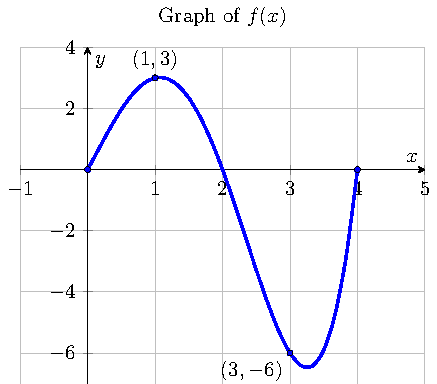
\includegraphics[width=0.9\columnwidth]{figures/0-1-act1.pdf}
\end{center}
\end{minipage}
\begin{minipage}{0.5\columnwidth}
\ba
\item What is the domain of $f(x)$?
\item Approximate the range of $f(x)$.
\item What are  $f(0)$, $f(1)$, $f(3)$, $f(4)$, and $f(5)$?
\ea
\end{minipage}

\end{activity}
\begin{smallhint}
    \ba
        \item The domain is the collection of possible $x$ values.
        \item The range is the collection of possible $y$ values.
        \item Find the $y$ values for each of the given $x$ values.
    \ea
\end{smallhint}
\begin{bighint}
    \ba
        \item The domain should be written as $?? \le x \le ??$.  Look for the smallest
            and largest possible $x$ values.
        \item The range should be written as $?? \le y \le ??$.  Approximate the smallest
            and largest possible $y$ values.
        \item Find the $y$ values for each of the given $x$ values.
    \ea
\end{bighint}
\begin{activitySolution}
   \ba
        \item The domain of $f(x)$ is $0 \le x \le 4$.
        \item The approximate range of $f(x)$ is $-7 \le y \le 3$.  Without the function
            itself we cannot be sure of the actual heights of the function at the maximum
            and the minimum.
        \item $f(0) = 0$, $f(1) = 3$, $f(3) = -6$, $f(4) = 0$, and $f(5)$ does not exist
            since $5$ is not in the domain of $f(x)$.
   \ea
\end{activitySolution}
\aftera
